\documentclass[spanish,12pt,a4paper,titlepage]{article}
\usepackage[latin1]{inputenc}
\usepackage{graphicx}
\usepackage{subfig}
\usepackage{wrapfig}
\usepackage{multirow}
\usepackage{caption}
\usepackage{babel}
\usepackage[dvips]{hyperref}
\usepackage{amssymb}
\usepackage{listings}
\usepackage{epsfig}
\usepackage{amsmath}
%\usepackage[Lenny]{sty/fncychapleo}

\setlength{\topmargin}{-1.5cm}
\setlength{\textheight}{25cm}
\setlength{\oddsidemargin}{0.3cm} 
\setlength{\textwidth}{15cm}
\setlength{\columnsep}{0cm}

\begin{document}


\part{Modelo F�sico}

Resulta imprescindible para controlar el quadcopter comprender cabalmente su comportamiento. Con esta �ptica, lo que se busca es obtener el modelo m�s sencillo que sea capaz de representar adecuadamente al sistema. El objetivo de esta secci�n es el de realizar el desarrollo de dicho modelo. La forma de modelar el sistema elegida es un Modelo de Variables de Estado, de ahora en m�s MVE.

Al tratarse de una plataforma comercial no se tienen datos sobre algunos de los par�metros fundamentales para el desarrollo de dicho modelo. Por ejemplo, no se conoce como es la respuesta de los motores (tanto velocidad como empuje), el tensor de inercia del sistema,etc. Por lo tanto dividiremos el an�lisis del modelo en varias etapas. La primera de ellas consiste en obtener las constantes del sistema, luego se procede a caracterizar la respuesta de los motores, a continuacion se  desarrolla el  modelo te�rico, finalmente en la �ltima secci�n se presentan los resultados obtenidos con dicho modelo y se contrastan con la realidad.    

\section{Constantes del sistema}

\section{Caracterizaci�n de los motores}


\section{Desarrollo te�rico}

\subsection{Sistema de Referencia}

A lo largo del presente desarrollo se trabajar� constantemente con dos sistemas de referencia; uno inercial\footnote{En esta secci�n se consideran sistemas inerciales en el sentido cl�sico} solidario a la tierra ($S_I$) y otro solidario al quadcopter ($S_q$). El sistema $S_q$ se puede obtener realizando tres rotaciones compuestas del sistema $S_I$, dichas rotaciones se muestran en la figura \ref{fig:rotaciones}. 

\begin{figure} [h!]
  \centering
  \subfloat[Rotaci�n seg�n eje $\hat{k}$]{\label{fig:angulos_1}
  		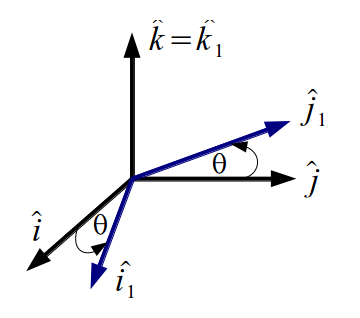
\includegraphics[width=0.3\textwidth]
  			{./Pics/angulos_1.png}}
  \subfloat[Rotaci�n seg�n eje $\hat{j}$]{\label{fig:angulos_2} 
  		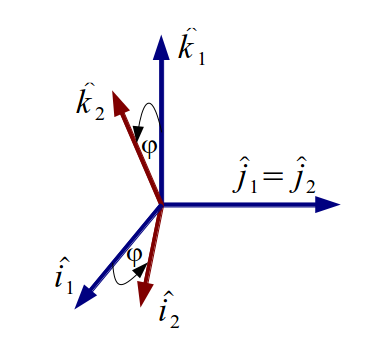
\includegraphics[width=0.3\textwidth]
  			{./Pics/angulos_2.png}}
  \subfloat[Rotaci�n seg�n eje $\hat{i}$]{\label{fig:angulos_3} 
  		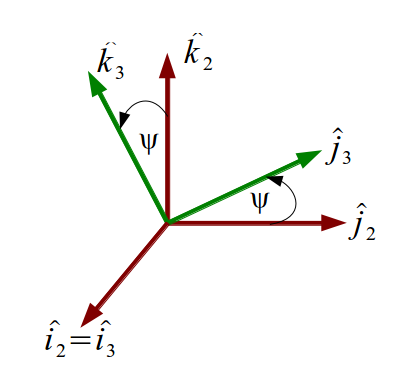
\includegraphics[width=0.3\textwidth]
  			{./Pics/angulos_3.png}}
  \caption{Rotaciones}
  \label{fig:rotaciones}
\end{figure}

La importancia del sistema $S_q$ radica en las simplificaciones que introduce a la hora de escribir las ecuaciones, ya que por ejemplo en dicho sistema el empuje de las helices, los torques que introducen y velocidades angulares de los motores del quadcopter tienen siempre la misma direcci�n. 

%TODO experto en paint tiene que hacer los propios dibujos
Las tres transformaciones pueden reprsesentarse matricialmente de la siguiente forma: 


\begin{small}


$H_I^1=\left(\begin{array}{ccc}
  \cos\theta&\sin\theta&0\\
  -\sin\theta&\cos\theta&0\\
  0&0&1\\
  \end{array}\right)   H_1^2=\left(\begin{array}{ccc}
  \cos\phi&0&\sin\phi\\
  0&1&0\\
  -\sin\phi&0&\cos\phi\\
  
  \end{array}\right)  H_2^q=\left(\begin{array}{ccc}
   1&0&0\\  
  0&\cos\psi&\sin\psi\\
  0&-\sin\psi&\cos\psi\\
  
  \end{array}\right) $\\


\end{small}  
La transformacion de las coordenadas del sistema inercial al sistema solidario al quadcopter se obtiene realizando el producto de las tres matrices de rotacion definidas.\\

\begin{scriptsize}
$H_I^q=H_I^1.H_1^2.H_2^q=\left(\begin{array}{ccc}
\cos\phi\cos\theta& \cos\phi\sin\theta& \sin\phi\\
-\cos\psi\sin\theta - \cos\theta\sin\phi\sin\psi&\cos\psi\cos\theta - \sin\phi\sin\psi\sin\theta& \cos\phi\sin\psi\\
\sin\psi\sin\theta - \cos\psi\cos\theta\sin\phi& - \cos\theta\sin\psi - \cos\psi\sin\phi\sin\theta& \cos\phi\cos\psi\\
\end{array} \right)$
\end{scriptsize}
 
Adem?as de la relacion entre las coordenadas de un sistema y del otro, es �til conocer la relacion que existe entre la velocidad angular del sistema y las derivadas de los angulos de euler. 
Por como fue construido el sistema de referencia solidario al quadcopter, se deduce trivialmente que la velocidad angular del mismo se puede escribir como:\\

$\vec{\omega}=w_{q1}\vec{i_q}+w_{q2}\vec{j_q}+w_{q3}\vec{k_q}=\dot{\theta}\vec{k}+\dot{\phi}\vec{j_1}+\dot{\psi}\vec{i_2}$\\

Al realizar la �ltima rotaci?on el vector $\vec{i_2}$ no se modifica. Por otra parte, multiplicando los vectores $\vec{k}$ y $\vec{j_1}$ por las matrices $H_1^2.H_2^q$ y $H_2^q$ respectivamente se puede obtener la velocidad angular del quadcopter en el sistema de coordenadas referido a el. Lo que tenemos entonces es:\\

\begin{footnotesize}

$\vec{\omega}=w_{q1}\vec{i_q}+w_{q2}\vec{j_q}+w_{q3}\vec{k_q}= (\dot{\psi}  +    \dot{\theta}\sin\phi)\vec{i_q}+(\dot{\phi}\cos\psi + \dot{\theta}\cos\phi \sin\psi)\vec{j_q}+(\dot{\theta}\cos\phi \cos\psi -  \dot{\phi}\sin\psi)\vec{k_q}$\\


\end{footnotesize}

De esta ecuaci?on se obtienen tres relaciones entre las velocidades angulares respecto de cada eje principal del sistema de coordenadas solidario al quadcopter con las derivadas de los angulos de euler. Podemos re escribir dicha ecuaci�n de la siguiente forma: \\

$\left(\begin{array}{c}
\dot{\psi}\\
\dot{\phi}\\
\dot{\theta}\\
\end{array}\right)=\left(\begin{array}{c}
\omega_{q1} - \omega_{q3}\tan\phi \cos\psi - \omega_{q2}\tan\phi \sin\psi\\
\omega_{q2}\cos \psi - \omega_{q3}\sin\psi\\
\omega_{q3} \frac{\cos\psi}{\cos\phi}  + \omega_{q2}\frac{\sin\psi}{\cos\phi} \\
\end{array}\right)$\\

Detendremos en este punto el analisis cinematico para considerar la dinamica del mismo. Para resolver el problema de la dinamica del sistema se consideran las ecuaciones cardinales.

\subsection{Primera Cardinal}
 
La primer cardinal indica que en un sistema inercial la suma de las fuerzas externas a un objeto es igual a su masa total por su aceleracion. Esto se puede escribir:
\begin{large}
\\$\sum \vec{F_{ext}} = M\vec{a}$\\
\end{large}


El vector aceleracion no es otra cosa que la derivada segunda del vector posici?on del centro de masa. Por lo tanto se tiene que $\vec{a} = \ddot{x}\vec{i}+\ddot{y}\vec{j}+\ddot{z}\vec{k}$. Las fuerzas que actuan sobre el sistema son los empujes de cada turbina y el peso. Los empujes ($T_i$ con $i=1..4$) son en el sentido de $\vec{k_q}$ mientras que el peso es en el sentido de $\vec{k}$. Para obtener el empuje de los motores en el sistema $S_I$ alcanza con realizar el cambio de base del sistema $S_q$ al sistema inercial. El empuje de los motores puede escribirse como:

\begin{large}


$\sum_{i=1}^{i=4}T_i=\sum_{i=1}^{i=4}T_iH_I^q\left(\begin{array}{c}
0\\
0\\
1\\
\end{array} \right)$
\end{large}

Operando, se puede reescribir la primer cardinal de la siguiente forma:\\

\begin{large}

$\left(\begin{array}{c}\ddot{x}\\
\ddot{y}\\
\ddot{z}\\
\end{array} \right) = \frac{1}{M}\left[\left(\begin{array}{c}
\sin\psi \sin\theta - \cos\psi \cos\theta \sin\phi	\\
-\cos\theta \sin\psi - \cos\psi \sin\phi \sin\theta\\
\cos\phi \cos\psi\\
\end{array}\right) - g\left(\begin{array}{c}
0\\
0\\
1\\

\end{array}\right)\right]$


\end{large}

\subsection{Segunda Cardinal}

La segunda cardinal indica que la derivada del momento angular de un sistema respecto a un punto (Q) es igual al torque externo que se ejerce sobre el mismo m�s un t�rmino que depende de la velocidad de dicho punto. La ecuaci�n queda:\\


\begin{large}

$\frac{d\vec{L_Q}}{dt} =M_Q^{ext}+M\vec{v_G}\ \times \dot{\vec{r_Q}} $\\

\end{large}

Asumiendo simetr�a del sistema, se puede considerar que el centro de masa del sistema se encuentra en el centro de la esfera principal del mismo. Esto no es completamente cierto ya que la bater�a del UAV queda por fuera de la esfera y los apoyos tambi�n, sin embargo se puede asume en una primera aproximaci�n del modelo que si lo es.De esta forma si planteamos la segunda cardinal en el centro de masa obtenemos:\\

\begin{large}

$\frac{d\vec{L_G}}{dt} =M_G^{ext}$\\
\end{large} 

Si nombramos a las turbinas como se observa en el esquema \ref{fig:		} se obtiene rapidamente que: 

\begin{large}
$M_G^{ext} = L\left(\begin{array}{c}
T3-T1\\
T2-T4\\
0\\
\end{array} \right)$
\end{large}

Por otra parte el momento angular del sistema se compone del momento angular del quadcopter y de cada motor. Consideraremos el quadcopter sin los motores como un primer rigido y los motores cada uno como un rigido independiente.

EL momento angular de un r�gido respecto a un punto Q puede calcularse como:\\

\begin{large}
$\vec{L_{Q_i}} = M_i(\vec{G_i-Q})\times\vec{V_Q}+\Pi_{Q_i}\vec{\Omega_i}$\\
\end{large}  

Donde $M_i$, $G_i$, $\Pi_{Q_i}$ y $\vec{\Omega_i}$ son la masa de cada rigido, su centro de masa, su tensor de inercia y su velocidad angular respectivamente.

Como se propuso anteriormente, se elije calcular el momento angular en el centro de masa del quadcopter. Asumiendo que los cuatro motores son id�nticos podemos escribir el momento angular del quadcopter sin los motores como:\\

\begin{large}
$\vec{L_{G_q}} = (M-4 M_m)(\vec{G-G})\times\vec{V_G}+\Pi_{G_q}\vec{w_q}=\Pi_{G_q}\vec{\omega_q}$\\

\end{large} 

Del mismo modo el momento angular del primer motor queda:\\

\begin{large}
$\vec{L_{G_{m1}}} = M_m L\vec{x\prime}\times\vec{V_G} + \Pi_{G_{m1}}\vec{\Omega_i} $\\
\end{large}

Por la configuraci�n del sistema se observa que al sumar el primer t�rmino de cada momento angular de los motores el resultado es cero. Por otra parte la velocidad angular de cada motor es $\vec{\Omega_i} = \vec{\omega_q}+\omega_i\vec{k\prime}$, donde $\omega_i$ es la velocidad con la que gira cada motor respecto de su eje principal. Nuevamente asumiendo que todos los motores son id�nticos se tiene:\\

\begin{large}
$\vec{L_G} =\Pi_{G_q}\vec{\omega_q}+\Pi_{G_{m}}(4\vec{\omega_q}+\sum_{i=1}^{i=4}\omega_i\vec{k\prime})=(\Pi_{G_q}+4\Pi_{G_{m}})\vec{\omega_q}+\Pi_{G_{m}}\sum_{i=1}^{i=4}\omega_i\vec{k\prime} $\\
\end{large}

Uno de los t�rminos de la segunda cardinal es la derivada del momento angular. Tanto los tensores de inercia como las velocidades angulares se encuentran expresadas en el sistema relativo. Para realizar dicha derivada se puede utilizar la siguiente f�rmula:\\

\begin{large}
$\frac{d\vec{A}}{dt} =\frac{d\prime\vec{A}}{dt}+\vec{\Omega}\times\vec{A} $\\\
\end{large}

En la ecuaci�n anterior $\frac{d}{dt}$ representa la derivada temporal, mientras que $\frac{d\prime}{dt}$ representa la derivada temporal respecto del sistema m�vil. Por otra parte $\vec{\Omega}$ es la velocidad angular del sistema m�vil respecto al inercial. Lo que se obtiene de dicha derivada es:\\

$\frac{d\vec{L_Q}}{dt} = (\Pi_{G_q}+4\Pi_{G_{m}})\dot{\vec{\omega_q}} +\Pi_{G_{m}}\sum_{i=1}^{i=4}\dot{\omega_i}\vec{k\prime}+\vec{\omega_q}\times((\Pi_{G_q}+4\Pi_{G_{m}})\vec{\omega_q}+\Pi_{G_{m}}\sum_{i=1}^{i=4}\omega_i\vec{k\prime} )$\\

En la ecuaci�n anterior se puede hacer la siguiente simplificaci�n: $\Pi_G = (\Pi_{G_q}+4\Pi_{G_{m}})$, donde $\Pi_G$ es el momento de inercia de todo el sistema en su centro de masa. 

A partir del c�lculo de esta derivada y de los momentos externos hallados anteriormente, podemos escribir la segunda cardinal. Operando con dicha ecuaci�n se la puede llevar a la forma:\\

\begin{huge}
ASUMO QUE LOS TENSORES DE INERCIA SON TODOS DIAGONALES\\
\end{huge}

$\left(\begin{array}{c}
\dot{\omega_{q1}}\\
\dot{\omega_{q2}}\\
\dot{\omega_{q3}}\\
\end{array}\right) = \left(\begin{array}{c}
\frac{\omega_{q2}\omega_{q3}(I_{yy}-I_{zz})+(T_3-T_1)+\omega_{q2}I_{zz_m}(\omega_1+\omega_2+\omega_3+\omega_4)}{I_{xx}}\\

\frac{\omega_{q1}\omega_{q3}(-I_{xx}+I_{zz})+(T_2-T_4)+\omega_{q1}I_{zz_m}(\omega_1+\omega_2+\omega_3+\omega_4)}{I_{yy}}\\

\frac{\omega_{q1}\omega_{q2}(I_{xx}-I_{yy})-I_{zz_m}(\dot{w_1}+\dot{w_2}+\dot{w_3}+\dot{w_4})}{I_{zz}}\\

\end{array}\right)$

 
\subsection{Modelo en variables de Estado}
\subsection{Algunas consideraciones adicionales sobre el modelo}

\end{document}

Algunos layouts para poner im�gnenes. Copien y peguen no
m�s. Hay figura com�n, dos figuras en 1 onda fig 3a y 3b, wrapfigures y una matriz de figuras. Ta bueno, todas quedan lindas y andan bien.

\begin{figure}[h!]
	\centering
	\includegraphics[width=0.75\textwidth]{./Pics/		.eps}
	\caption{		}
	\label{fig:		}
\end{figure}

\begin{figure} [h!]
  \centering
  \subfloat[caption 1]{\label{fig:		}
  		\includegraphics[width=0.45\textwidth]
  			{./Pics/		.eps}}
  \subfloat[caption 2]{\label{fig:		} 
  		\includegraphics[width=0.45\textwidth]
  			{./Pics/ 		.eps}}
  \caption{Caption general}
  \label{fig:	label general	}
\end{figure}

\begin{wrapfigure}{l}{0.6\textwidth}
  \vspace{-20pt}
  \begin{center}
    \includegraphics[width=0.45\textwidth]
    	{./Pics/		.eps}
  \end{center}
  \vspace{-20pt}
  \caption{		}
  \label{ 		}
  \vspace{-10pt}
\end{wrapfigure}

\begin{figure} [h!]
  \begin{center}
    \begin{tabular}{cc}
      \resizebox{50mm}{!}
      	{\includegraphics{./Pics/ 	.eps}} &
      \resizebox{50mm}{!}
      	{\includegraphics{./Pics/	.eps}} \\
      \resizebox{50mm}{!}
      	{\includegraphics{./Pics/	.eps}} &
      \resizebox{50mm}{!}
      	{\includegraphics{./Pics/	.eps}} \\
    \end{tabular}
    \caption{ 		}
    \label{ 		}
  \end{center}
\end{figure}